In this section, we first describe our experimental setup concerning both the instances we use as a benchmark as well as the hardware in use in \ref{eval: setup}.
\todo{rest of the stuff }

\subsection{Experimental Setup}
\label{eval: setup}
For our performance tests we utilize the same reduced IPC 2020 benchmark as in \cite{bretl2021parallel}, also giving our planners 900 seconds per instance. \\
Our tests were done on two machines. The first is a server with an Intel Xeon Gold 6138 processor with 4 sockets, 20 cores per socket and 2 threads per core clocked 2.00G Hz with around 750GB of RAM and running Ubuntu 20.04. We will call it PC1. The second is a server with an AMD EPYC 7702 processor with 1 socket with 64 cores and 2 threads per core clocked 2.00 GHz with around 1TB of RAM and running Ubuntu 20.04. We will call it PC2.

The performance tests were done on a server \\
We performed an additional test with an instrumented version of single-threaded CrowdHTN using random DFS and hash set based loop detection. The instrumentation allowed us to track information on the structure of our search graph and planner behavior, such as the prevalence of loops and search nodes created per second. This run was performed on the same set of instances as the performance test with up to 300 seconds per instance. The investigation was performed on a server with an AMD EPYC 7702 processor with 1 socket with 64 cores and 2 threads per core clocked 2.00 GHz with around 1TB of RAM and running Ubuntu 20.04.
\todo{describe machine used in malleability tests}

\paragraph{Naming Scheme}
As our CrowdHTN planner contains multiple configuration options, we use a succinct naming scheme to identify them in the evaluation. The name for a CrowdHTN configuration has the following structure:
\[
	\text{Cr}
	\left\langle \text{CrowdHTN version} \right\rangle
	\left\langle \# \text{of PEs} \right\rangle
	\left\langle \text{loop detection method} \right\rangle
	\left\langle \text{presence of restarts} \right\rangle
\]
A list of possible values for each category as well as their meaning is shown in table \ref{table: crowd configs}.
\begin{table}
	\caption{List of parameters identifying a CrowdHTN configuration}
	\label{table: crowd configs}
	\centering
	\begin{tabular}{|l|l|l|}
		\hline
		Parameter & Value & Meaning \\
		\hline
		CrowdHTN Version & O & Old CrowdHTN \\
		 			     & N & New CrowdHTN \\
		\hline
		Loop Detection Method & Hs & Hash Set \\
							  & Bl & Local Bloom Filter \\
							  & Bg & Global Bloom Filter \\
							  & No & No loop detection \\
		\hline
		Presence of Restarts & R & Time dependent restarts are used \\
							 & / & No time dependent restarts are used \\
		\hline
	\end{tabular}
\end{table}

\begin{comment}
CrowdHTN metadata
- same instance set
- 300 seconds per instance
- log the run time behavior regarding the search behavior
- 64 cores, 2 GHz max
- AMD EPYC 7702
- around 1 TB of RAM
- Ubuntu 20.04
\end{comment}

\subsection{Optimizations in CrowdHTN}
\label{eval: crowd optimizations}
In \ref{impl: reduce nodes} we described an improvement to our progression search which let us reduce the number of search nodes we instantiate. To evaluate the impact of this improvement we created an instrumented version of CrowdHTN which let us track this information during planning. We ran this version of CrowdHTN on our benchmark on PC2, using 1 PE, DFS and hash set based loop detection while giving it 300 seconds per instance. We tracked the metadata for all instances, whether a plan was found or not. In addition to the information on actions and world states, we tracked the number of search nodes which were duplicates. The results are shown in table \ref{table: tohtn metadata}. \\
Compared to the other measures, the ratio of tasks which are actions is relatively consistent between domains. It varies from about one third to about two thirds of all tasks. The ratio is lowest for the Logistics-Learned-ECAI-16 domain at $28.2\%$ and highest for Rover-GTOHP at $66.83\%$. \\
When it comes to shared world states, results vary more. On 11 out of the 24 test domains, a world state is on average shared by less than 10 search nodes. This is lowest for the Snake domain with only $1.4$ search nodes per world state. On the other hand for 6 out of our 24 domains more than $1000$ search nodes share one world state, going as far as $\sim3.5 \times 10^8$ search nodes per world state for the Transport domain. \\
To sum these improvements up, our improved search node exploration is a clear benefit on all domains, reducing the number of search nodes we need to represent by at least $28\%$. Sharing world states is more mixed. While sharing is extreme on some domains, it does come at the cost of an additional pointer indirection which may be harmful on domains with little sharing. \\
Regarding loop detection, the results are similarly varied as with state sharing. On 7 out of 24 domains no duplicate nodes were encountered at all and on another 5 domains less than 1\% of nodes were duplicates. At the other end of the spectrum we have Minecraft-Player and Logistics-Learned-ECAI-16 with $\sim30\%$ and Factories-simple with $\sim44\%$ of duplicate nodes. We will return to these numbers in the evaluation of different loop detection techniques in \ref{eval: loop detection}.
\begin{table}
	\caption{Metadata about progression search on our benchmark}
	\label{table: tohtn metadata}
	\centering
	\begin{tabular}{|l|c|r|r|}
		\hline
		Domain & Action\% & State Sharing & Loop\% \\
		\hline
		AssemblyHierarchical & 49.71 & 4793.8 & 0.006\\
		Barman-BDI & 33.56 & 10.4 & 4.866\\
		Blocksworld-GTOHP & 50.80 & 6.1 & 0.000\\
		Blocksworld-HPDDL & 49.34 & 83.4 & 1.690\\
		Childsnack & 53.94 & 28800.6 & 0.000\\
		Depots & 45.11 & 7.3 & 2.790\\
		Elevator-Learned-ECAI-16 & 47.89 & 44.9 & 1.663\\
		Entertainment & 49.49 & 7.2 & 0.095\\
		Factories-simple & 31.09 & 2.3 & 43.815\\
		Freecell-Learned-ECAI-16 & 44.42 & 2.5 & 0.000\\
		Hiking & 65.24 & 2.6 & 12.508\\
		Logistics-Learned-ECAI-16 & 28.20 & 4.7 & 30.348\\
		Minecraft-Player & 32.21 & 4.4 & 29.896\\
		Minecraft-Regular & 31.34 & 3.4 & 0.000\\
		Monroe-Fully-Observable & 48.65 & 114.0 & 1.457\\
		Monroe-Partially-Observable & 48.29 & 106.6 & 3.418\\
		Multiarm-Blocksworld & 47.06 & 28.9 & 8.240\\
		Robot & 50.00 & 46207.3 & 0.002\\
		Rover-GTOHP & 66.83 & 3.5 & 0.000\\
		Satellite-GTOHP & 34.66 & 52.5 & 0.013\\
		Snake & 47.16 & 1.4 & 6.948\\
		Towers & 49.99 & 5409.3 & 0.000\\
		Transport & 36.98 & 347788104.5 & 0.000\\
		Woodworking & 49.83 & 21708.8 & 0.442\\
		\hline
	\end{tabular}
\end{table}

\subsection{Comparing to old CrowdHTN}
- we win overall
- we loose some coverage?!
- specifically in Freecell-Learned-ECAI-16 we have a performance degradation
- we win in overall IPC score
- the hit or miss nature of CrowdHTN has increased

\subsection{Search Algorithms}
\label{eval: algorithms}
In section \ref{improv: search algorithms} we presented four search algorithms that we implemented for CrowdHTN. Those algorithms are random DFS, heuristic DFS, A-star like and BFS. We have tested all four algorithms on our test instance set using 4 PEs and a local bloom filter without restarts for loop detection. The results of this test are visualized in figure \ref{figure: eval algorithm}, a summary of coverage and IPC score is presented in table \ref{table: eval algorithm}. \\
Overall, random DFS performed best, followed by heuristic DFS, A-star like search and finally BFS with our best algorithm, random DFS, solving almost twice as many instances and having twice the IPC score of our worst algorithm, BFS. Additionally, we observe a hit-or-miss behavior in both our DFS implementations where plans are either found almost immediately or not at all. Out of the 50 instances solved by random DFS, only 18 were solved in more than 1 and out of these 18 only 9 were solved in more than 10 seconds. BFS on the other hand solves 14 out of 30 instances in more than a second and 11 of these 14 in over 10 seconds. As such, while overall worse performing it does seem to scale better with runtime. \\
Comparing our two DFS-based approaches, we see that random DFS performs better than heuristic DFS guided by our heuristic from section \ref{improv: crowd heuristic}. We attribute this to the fact that we consciously limited our heuristic to information on the hierarchy available from the lifted instance to reduce the time spent on precomputation. Others, such as \cite{holler2020htn} argue that heuristics must utilize both hierarchy and world state information. Our findings corroborate this theory.

\begin{figure}
	\caption{Plotting the number of solved instances per run time for CrowdHTN using DFS, heuristic DFS, A-star like search and BFS}
	\label{figure: eval algorithm}
	\centering
	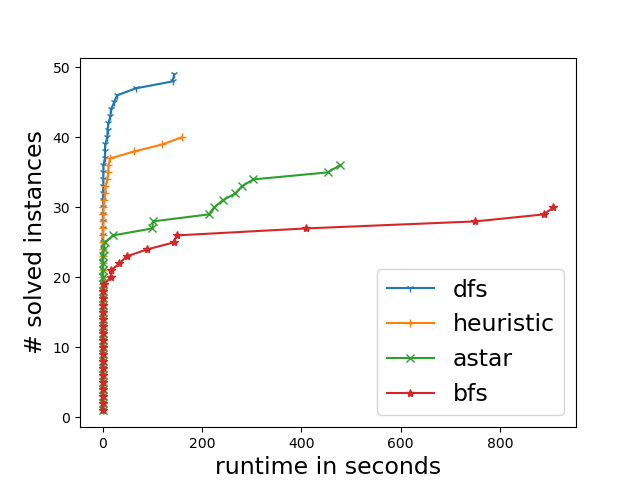
\includegraphics[width=0.5\textwidth]{images/final/search_algorithms.png}
\end{figure}
\begin{table}
	\caption{Coverage and IPC score of our search algorithms using 4 PEs and a local bloom filter}
	\label{table: eval algorithm}
	\centering
	\begin{tabular}{| l | r | r |}
		\hline
		Algorithm 		& Coverage & IPC Score \\
		\hline
		Random DFS 		& 41.7\%	& 43.09 \\ % 50
		Heuristic DFS 	& 33.3\%	& 35.60	\\ % 40
		A-star like 	& 38.3\%	& 27.13 \\ % 36
		BFS 			& 25.0\%	& 21.87	\\ % 30
		\hline
	\end{tabular}
\end{table}

\subsection{Local Loop Detection}
\label{eval: loop detection}
- general loop detection:
- performance of hash set vs bloom filter

- add runs without any loop detection to the evaluation
- split perf comparison on domains with and without loops
- table which gives us domain and loop percentage

- as bloom filters perform best, the rest of the evaluation will focus on them

\begin{figure}
	\caption{Plotting the number of solved instances per run time for CrowdHTN comparing hash set and local bloom filter based loop detection on 32 and 64 PEs}
	\label{figure: eval loop detection}
	\begin{subfigure}[b]{0.5\textwidth}
		\centering
		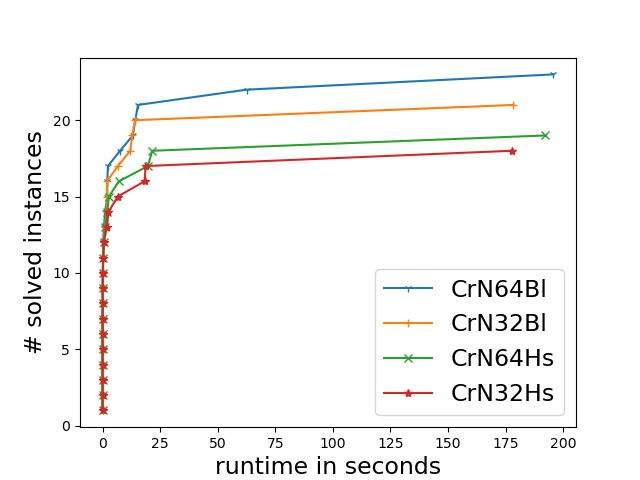
\includegraphics[width=\textwidth]{images/final/loop_detection_below_one}
		\caption{Instances with $< 1\%$ duplicate nodes}
	\end{subfigure}
	\begin{subfigure}[b]{0.5\textwidth}
		\centering
		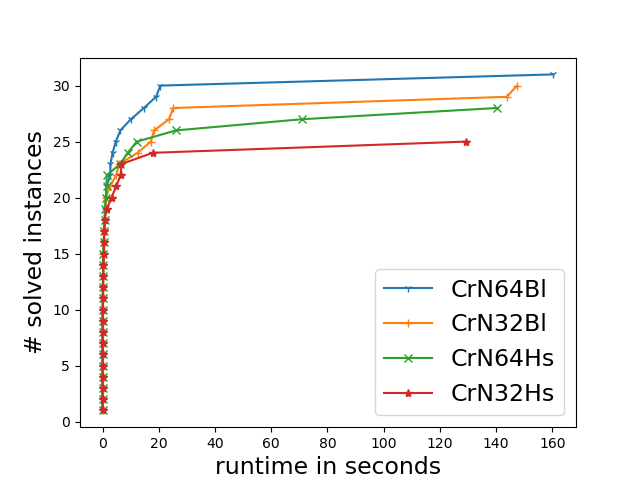
\includegraphics[width=\textwidth]{images/final/loop_detection_above_one}
		\caption{Instances with $> 1\%$ duplicate nodes}
	\end{subfigure}
	
	% python3 ../MA_scripts/diagrams.py -files=results_64_dfs_local_bloom_handlepanic_1.csv,results_32_dfs_local_bloom_handlepanic.csv,results_64_dfs_local_hashset_handlepanic.csv,results_32_dfs_local_hashset_handlepanic.csv -names=64-bloom,32-bloom,64-hashset,32-hashset
\end{figure}

\begin{table}
	\caption{Coverage and IPC score while using hash set and local bloom filter based loop detection on 32 and 64 PEs}
	\label{table: eval loop detection}
	\centering
	\begin{tabular}{| l | r | r |}
		\hline
		Configuration & Coverage & IPC Score \\
		\hline
		Bloom, 64 PEs		& 45.0\%	& 47.37 \\ % 54
		Bloom, 32 PEs		& 42.5\%	& 44.24 \\ % 51
		Hash set, 64 PEs	& 39.2\%	& 41.84 \\ % 47
		Hash set, 32 PEs	& 35.8\%	& 38.71 \\ % 43
		\hline
	\end{tabular}
\end{table}

\subsection{Probabilistic Restarts}
\label{eval: restarts}
- test the probabilistic restarts
- with 900 seconds we expect $\sum_{t=1}^{899} \frac{1}{t} \approx 7.38$ restarts per run
- expect coverage to go up, IPC score to go slightly down
- we are expecting many restarts especially at the beginning, this will lower scores on easy instances
- however, we also expect the restarts to somewhat negate the hit-or-miss nature of our planner, leading to increased coverage

\begin{figure}
	\caption{Evaluating CrowdHTN with a local bloom filter with and without restarts}
	\label{figure: restarts}
	\centering
	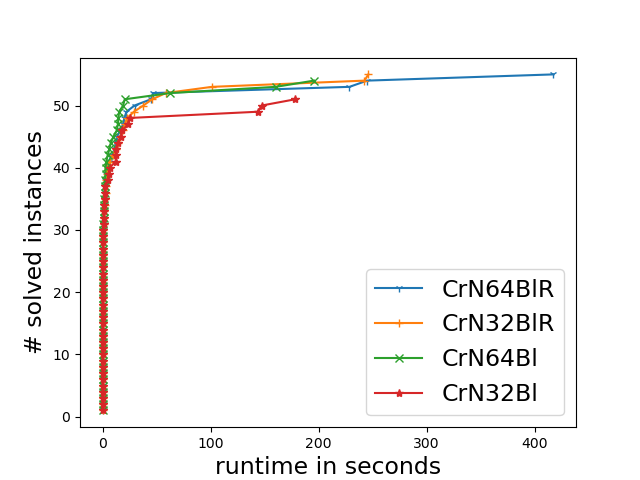
\includegraphics[width=0.5\textwidth]{images/final/restarts}
\end{figure}
\todo{}

\subsection{Global Loop Detection}
\label{eval: global loop}
- test the global loop detection with restarts on 32 and 64 PEs on our full benchmark
- 
\begin{figure}
	\caption{Comparing CrowdHTN with a local bloom filter and restarts with global loop detection}
	\label{figure: global loops}
	\centering
	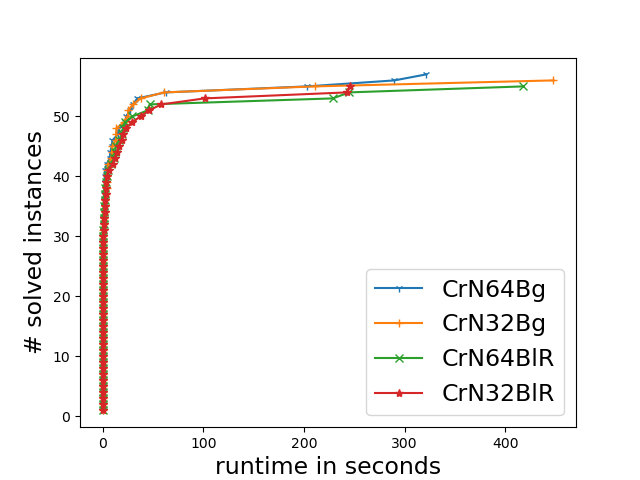
\includegraphics[width=0.5\textwidth]{images/final/global_loops}
\end{figure}

\subsection{Scalability of CrowdHTN}
\label{eval: scalability}
In general, the scaling behavior of CrowdHTN is hard to visualize due to it's nature as a search based planner using DFS. As a result, instances tend to either be solved extremely fast even on few PEs or not solved at all even as we increase the available resources. To demonstrate scaling, we want instances that are reliably solved on any number of PEs but which are not trivial. Looking at our previous benchmarks 

- demonstrating the scaling behavior of CrowdHTN is hard due to the hit-or-miss of random DFS in TOHTN
- we need an instance that is reliably solved
- we need an instance that takes long enough to solve to demonstrate an effect
- Monroe Fully Observable is such an instance
- separate test on i10pc137 (mention again what it is like, CPU etc)
- show scaling on a nice instance

\begin{figure}
	\caption{Plotting the number of solved instances per run time for CrowdHTN using DFS and a local bloom filter on 64, 16 and 4 PEs}
	\label{figure: eval scalability}
	\centering
	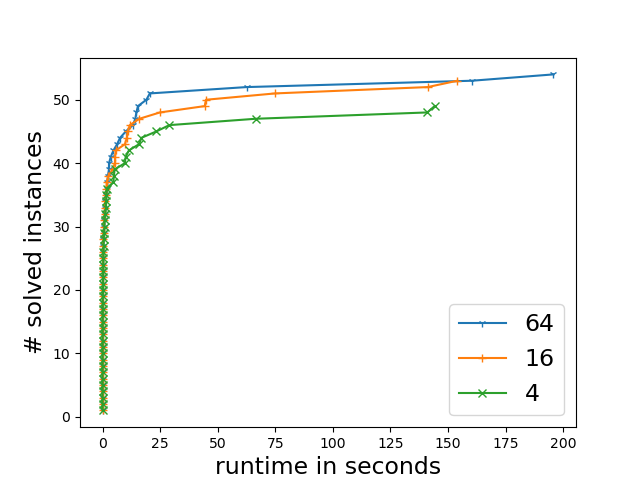
\includegraphics[width=0.5\textwidth]{images/final/scalability}
	% python3 ../MA_scripts/diagrams.py -files=results_64_dfs_local_bloom.csv,results_16_dfs_local_bloom.csv,results_4_dfs_local_bloom.csv  -names=64,16,4
\end{figure}

\begin{table}
	\caption{Evalutating CrowdHTN on 20 instances of the Monroe-Fully-Observable domain}
	\label{table: eval scalability}
	\centering
	\begin{tabular}{|l|rc|rc|rc|rc|rc|rc|}
		\hline
		& \multicolumn{2}{c|}{\textbf{BL4}} & \multicolumn{2}{c|}{\textbf{BL16}} & \multicolumn{2}{c|}{\textbf{BL64}} & \multicolumn{2}{c|}{\textbf{BG4}} & \multicolumn{2}{c|}{\textbf{BG16}} & \multicolumn{2}{c|}{\textbf{BG64}}\\
		& Time & IPC & Time & IPC & Time & IPC & Time & IPC & Time & IPC & Time & IPC\\
		\hline
		01 & 0.2 & 1.00 & 0.1 & 1.00 & 0.4 & 1.00 & 0.1 & 1.00 & 0.7 & 1.00 & 0.1 & 1.00\\
		02 & 161.5 & 0.25 & 30.7 & 0.50 & 1.3 & 0.96 & 115.6 & 0.30 & 10.5 & 0.65 & 22.6 & 0.54\\
		03 & / & 0.00 & 5.7 & 0.74 & 8.4 & 0.69 & 250.5 & 0.19 & 4.0 & 0.80 & 30.5 & 0.50\\
		04 & 0.4 & 1.00 & 0.3 & 1.00 & 0.2 & 1.00 & 0.3 & 1.00 & 0.3 & 1.00 & 0.4 & 1.00\\
		05 & 49.9 & 0.43 & 55.6 & 0.41 & 22.6 & 0.54 & 23.7 & 0.53 & 30.2 & 0.50 & 26.6 & 0.52\\
		06 & 183.9 & 0.23 & 60.1 & 0.40 & 3.5 & 0.82 & 129.0 & 0.29 & 61.7 & 0.39 & 18.2 & 0.57\\
		07 & 18.5 & 0.57 & 7.2 & 0.71 & 3.2 & 0.83 & 5.3 & 0.75 & 2.0 & 0.90 & 4.0 & 0.80\\
		08 & 98.1 & 0.33 & 48.0 & 0.43 & 4.4 & 0.78 & 108.0 & 0.31 & 101.7 & 0.32 & 12.5 & 0.63\\
		09 & 62.3 & 0.39 & 17.7 & 0.58 & 26.0 & 0.52 & 70.8 & 0.37 & 13.5 & 0.62 & 14.3 & 0.61\\
		10 & 122.1 & 0.29 & 33.9 & 0.48 & 23.8 & 0.53 & 80.4 & 0.35 & 61.9 & 0.39 & 11.0 & 0.65\\
		11 & 148.9 & 0.26 & 60.5 & 0.40 & 15.7 & 0.60 & 148.6 & 0.26 & 62.8 & 0.39 & 15.0 & 0.60\\
		12 & 137.5 & 0.28 & 47.9 & 0.43 & 19.4 & 0.56 & 223.4 & 0.20 & 34.7 & 0.48 & 25.6 & 0.52\\
		13 & 19.4 & 0.56 & 2.7 & 0.85 & 1.5 & 0.94 & 7.9 & 0.70 & 0.6 & 1.00 & 1.7 & 0.92\\
		14 & 171.3 & 0.24 & 61.1 & 0.40 & 36.1 & 0.47 & 279.5 & 0.17 & 36.2 & 0.47 & 42.1 & 0.45\\
		15 & / & 0.00 & 6.5 & 0.73 & 4.3 & 0.79 & / & 0.00 & 5.0 & 0.76 & 0.8 & 1.00\\
		16 & / & 0.00 & 6.3 & 0.73 & 2.0 & 0.90 & 7.1 & 0.71 & 6.2 & 0.73 & 4.8 & 0.77\\
		17 & / & 0.00 & 1.6 & 0.93 & 11.2 & 0.64 & / & 0.00 & / & 0.00 & 1.8 & 0.91\\
		18 & 16.7 & 0.59 & 40.0 & 0.46 & 10.3 & 0.66 & 47.2 & 0.43 & 9.0 & 0.68 & 37.7 & 0.47\\
		19 & 1.9 & 0.90 & 5.1 & 0.76 & 1.8 & 0.91 & 15.7 & 0.60 & 15.0 & 0.60 & 5.7 & 0.74\\
		20 & 21.7 & 0.55 & 2.9 & 0.84 & 2.5 & 0.86 & 12.5 & 0.63 & 6.0 & 0.74 & 4.6 & 0.78\\
		\hline
		& & 7.88 & & 12.78 & & 15.01 & & 8.81 & & 12.43 & & 13.98\\
		\hline
	\end{tabular}
\end{table}

\subsection{Malleable CrowdHTN}
\label{eval: malleable}
To test the behavior of CrowdHTN under malleable conditions, we want to again focus on a problem instance which shows good scalability. In the previous discussion on CrowdHTN scalability we focused on the Monroe-Fully-Observable domain. We will continue using this domain, specifically problem 11. We performed our test using 32 PEs and trying to solve the instance 100 times. Our job on problem 11, which we will call the main job, had priority 1 and a wallclock time limit of 90 seconds. Every 20 seconds we injected an unsolvable job with priority 1 and a wallclock time limit of 10 seconds. This means the main job oscillates every 10 seconds from having 32 to having 16 PEs available and back. We compare both the coverage and the average run time of those instances with moldable CrowdHTN using 16, 24 and 32 PEs. The results are listed in table \ref{table: malleability}. Figure \ref{figure: malleability} shows a box plot of run times per solver. \\
- the tail of the run times is lost
- we expect 4 restarts by 30 seconds
- we expect only one more by the time 90 seconds have passed
- there seems to be some loss as the number of PEs is reduced and increases again
- we send the root off to a random other PE, may loose information if the reduction in PEs is large and we send it to a PE which was also just taken away

\begin{table}
	\caption{Coverage and average run time of malleable and moldable CrowdHTN}
	\label{table: malleability}
	\centering
	
	\begin{tabular}{|l|c|c|}
		\hline
		Configuration & Coverage & Average run time in seconds \\
		\hline
		Malleable, average 24 PEs	& 66\%	& 28.98 \\
		Moldable 16 PEs				& 93\%  & 45.73 \\
		Moldable 24 PEs				& 97\%  & 36.62 \\
		Moldable 32 PEs				& 98\%  & 25.98 \\
		\hline
	\end{tabular}
\end{table}
\begin{figure}
	\caption{Distribution of solving times for malleable and moldable CrowdHTN}
	\label{figure: malleability}
	\centering
	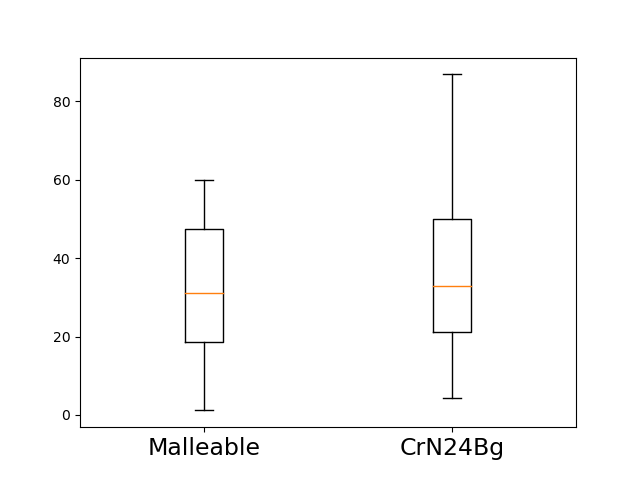
\includegraphics[width=0.5\textwidth]{images/final/malleability}
\end{figure}

\subsection{Conclusion}
\label{eval: conclusion}
- final discussion stuff

Things to plot:
- old Crowd on 4, 16, 64 cores
- new Crowd on 4, 16, 64 cores
- new Crowd with bloom filter, hash set and without ld, 32, 64
- new Crowd with bloom filter with(out) restarts, 32, 64
- new Crowd with global loop detection
- sequential planners HyperTensioN and PANDA
- Malleable vs non moldable Crowd

\begin{table}
	\caption{Domain-wise comparison of the old and improved moldable CrowdHTN}
	\label{table: eval old new}
	
	%python3 table_maker.py -results=../evaluation/final_run_data/WorSt_DFS_p4_loop.csv,../evaluation/final_run_data/WorSt_DFS_p16_loop.csv,../evaluation/final_run_data/WorSt_DFS_p64_loop.csv,../experimental_results/results_4_dfs_local_bloom.csv,../experimental_results/results_16_dfs_local_bloom.csv,../experimental_results/results_64_dfs_local_bloom_handlepanic_1.csv -planner_names=CrO4Hs,CrO16Hs,CrO64Hs,CrN4Bl,CrN16Bl,CrN64Bl -out_file=table.txt
	
	\begin{adjustbox}{angle=90}
	
	\begin{tabular}{|l|cc|cc|cc|cc|cc|cc|}
		\hline
		& \multicolumn{2}{c|}{\textbf{CrO4Hs}} & \multicolumn{2}{c|}{\textbf{CrO16Hs}} & \multicolumn{2}{c|}{\textbf{CrO64Hs}} & \multicolumn{2}{c|}{\textbf{CrN4Bl}} & \multicolumn{2}{c|}{\textbf{CrN16Bl}} & \multicolumn{2}{c|}{\textbf{CrN64Bl}}\\
		Domain & IPC & Cov & IPC & Cov & IPC & Cov & IPC & Cov & IPC & Cov & IPC & Cov\\
		\hline
		AssemblyHierarchical & \textbf{1.0} & 20\%  & \textbf{1.0} & 20\%  & 0.98 & 20\%  & \textbf{1.0} & 20\%  & \textbf{1.0} & 20\%  & \textbf{1.0} & 20\%  \\
		Barman-BDI & 1.79 & 40\%  & 1.78 & 40\%  & 1.74 & 40\%  & \textbf{2.0} & 40\%  & \textbf{2.0} & 40\%  & 1.97 & 40\%  \\
		Blocksworld-GTOHP & 2.0 & 40\%  & 1.99 & 40\%  & \textbf{2.49} & 60\%  & 2.0 & 40\%  & 2.0 & 40\%  & 2.39 & 60\%  \\
		Blocksworld-HPDDL & \textbf{3.21} & 80\%  & 3.14 & 80\%  & 3.01 & 80\%  & 3.03 & 80\%  & 3.02 & 80\%  & 2.98 & 80\%  \\
		Childsnack & 2.6 & 80\%  & 2.55 & 80\%  & 2.37 & 80\%  & \textbf{2.96} & 80\%  & 2.93 & 80\%  & 2.82 & 80\%  \\
		Depots & 3.63 & 80\%  & 3.72 & 80\%  & 3.6 & 80\%  & \textbf{3.92} & 80\%  & 3.86 & 80\%  & 3.85 & 80\%  \\
		Elevator-Learned-ECAI-16 & 4.06 & 100\%  & 4.03 & 100\%  & 3.86 & 100\%  & 4.33 & 100\%  & \textbf{4.36} & 100\%  & 4.29 & 100\%  \\
		Entertainment & 0.0 & 0\%  & 0.0 & 0\%  & 0.0 & 0\%  & 0.0 & 0\%  & 0.0 & 0\%  & 0.0 & 0\%  \\
		Factories-simple & 1.91 & 40\%  & \textbf{1.93} & 40\%  & 1.86 & 40\%  & 1.0 & 20\%  & 1.0 & 20\%  & 1.0 & 20\%  \\
		Freecell-Learned-ECAI-16 & 0.0 & 0\%  & 0.0 & 0\%  & 0.0 & 0\%  & 0.0 & 0\%  & 0.0 & 0\%  & 0.0 & 0\%  \\
		Hiking & \textbf{2.0} & 40\%  & 1.75 & 40\%  & 1.7 & 60\%  & \textbf{2.0} & 40\%  & \textbf{2.0} & 40\%  & \textbf{2.0} & 40\%  \\
		Logistics-Learned-ECAI-16 & 2.57 & 60\%  & \textbf{2.87} & 80\%  & 2.79 & 80\%  & 0.0 & 0\%  & 0.0 & 0\%  & 0.0 & 0\%  \\
		Minecraft-Player & 1.73 & 40\%  & 1.7 & 40\%  & 1.62 & 40\%  & \textbf{2.0} & 40\%  & \textbf{2.0} & 40\%  & \textbf{2.0} & 40\%  \\
		Minecraft-Regular & 3.14 & 80\%  & 3.1 & 80\%  & 2.99 & 80\%  & \textbf{3.6} & 80\%  & 3.58 & 80\%  & 3.5 & 80\%  \\
		Monroe-Fully-Observable & 1.68 & 100\%  & 2.45 & 100\%  & 2.07 & 100\%  & 1.92 & 60\%  & 3.3 & 100\%  & \textbf{4.08} & 100\%  \\
		Monroe-Partially-Observable & 0.93 & 20\%  & 0.0 & 0\%  & 0.82 & 20\%  & \textbf{1.0} & 20\%  & 0.0 & 0\%  & \textbf{1.0} & 20\%  \\
		Multiarm-Blocksworld & \textbf{1.0} & 20\%  & \textbf{1.0} & 20\%  & 0.98 & 20\%  & 0.0 & 0\%  & \textbf{1.0} & 20\%  & \textbf{1.0} & 20\%  \\
		Robot & \textbf{2.0} & 40\%  & \textbf{2.0} & 40\%  & \textbf{2.0} & 40\%  & \textbf{2.0} & 40\%  & \textbf{2.0} & 40\%  & \textbf{2.0} & 40\%  \\
		Rover-GTOHP & 3.7 & 100\%  & 3.62 & 100\%  & 3.26 & 80\%  & \textbf{4.56} & 100\%  & 4.55 & 100\%  & 4.47 & 100\%  \\
		Satellite-GTOHP & 0.0 & 0\%  & 0.0 & 0\%  & 0.0 & 0\%  & 0.0 & 0\%  & \textbf{1.0} & 20\%  & 0.0 & 0\%  \\
		Snake & 3.07 & 80\%  & 3.14 & 80\%  & 2.84 & 80\%  & 3.1 & 80\%  & \textbf{3.89} & 100\%  & 3.4 & 80\%  \\
		Towers & 2.2 & 60\%  & 2.2 & 60\%  & 2.15 & 60\%  & \textbf{2.66} & 60\%  & 2.65 & 60\%  & 2.61 & 60\%  \\
		Transport & 0.0 & 0\%  & 0.0 & 0\%  & 0.0 & 0\%  & 0.0 & 0\%  & 0.0 & 0\%  & \textbf{1.0} & 20\%  \\
		Woodworking & 0.0 & 0\%  & 0.0 & 0\%  & 0.0 & 0\%  & 0.0 & 0\%  & 0.0 & 0\%  & 0.0 & 0\%  \\
		\hline
		\textbf{Instances: 120} & 44.2 & 47\% & 44.0 & 47\% & 43.1 & 48\% & 43.1 & 41\% & 46.1 & 44\% & 47.4 & 45\% \\
		\hline
	\end{tabular}

	\end{adjustbox}
\end{table}
